\documentclass[oneside,12pt]{report}  

% the dimensions of the page
\textheight=9.25in \topmargin=-0.5in   %See note in Chapter 8 of Sample Report about "Page scaling" option in Adobe
\textwidth=6.0in
\oddsidemargin=0.3in
\evensidemargin=0.3in  % Needed to balance even and odd pages in twoside print copy
\usepackage{listings}



\usepackage{amssymb}
% Useful packages
\usepackage{dtklogos}
\usepackage{amsmath}
\usepackage{bm}
%\usepackage[colorlinks=true,pagebackref,linkcolor=blue]{hyperref}
\usepackage{amsfonts}
\usepackage{amsthm}
\usepackage{amsmath}
\usepackage{algorithm}
\usepackage{algorithmic}
\usepackage[marginal]{footmisc}
\usepackage{caption}
\usepackage{excludeonly}
\usepackage{float}
\usepackage{amssymb}
\usepackage{txfonts}
\usepackage{array}

%\usepackage{doc}
%% Following sets up logic and formatting for conditional twoside copying
%\usepackage{ifthen, color, fancyvrb}
%\usepackage{nextpage}\pagestyle{plain}
%\newcommand\myclearpage{\cleartooddpage
%  [\thispagestyle{empty}]
%  }

\DeclareMathOperator*{\argmin}{arg\ min}
\DeclareMathOperator*{\sign}{sign}

% Note special alternative codes for using TWO bibliographies; see cautionary note in
\DeclareGraphicsExtensions{ps,eps,PNG,png}

% Theorem-like command definitions:
\newtheorem{theorem}{Theorem}[chapter]
\newtheorem{lemma}{Lemma}[chapter]
\newtheorem{definition}{Definition}  % Note, this italicizes everything

% Print the chapter and sections in the toc
\setcounter{tocdepth}{1}

% Specify which files to typeset for this run (note that overall pagination is preserved)
%\includeonly{chapter1, chapter2}
% Specify which files NOT to typeset for this run (note that overall pagination is preserved)
%\excludeonly{}

% Groundwork for allowing double-sided copying with blank versos
\def\prefacesection#1{
\chapter*{#1}
\addcontentsline{toc}{chapter}{#1}
}
\usepackage{graphicx}
\graphicspath{{extra/}}
\begin{document}


\def\thefootnote{\fnsymbol{footnote}}

\thispagestyle{empty}

% The numbers below controls the amount of space between the following sections
\def\shiftdowna{0.32in}  % Adjust for balance
\def\shiftdownb{0.22in}  % Adjust for balance

% Set up the boiler plate at the top of the page

\begin{center}
\textbf{{\large Mathematical Modeling and Consulting }}\\

\vspace \shiftdowna

 
\includegraphics{jhu.png}\\


% Home Department
\vspace \shiftdowna
\underline {Sponsor}\\ 
\vspace{5pt}
\textbf{\large Stone \& Youngberg} \\
\vspace\shiftdowna
\textbf{{Final Report}}

% TITLE
\vspace \shiftdowna
\textbf{{\Large Constructing Dedicated Porfolio against District Bond Obligations from a Simplified Scenario}}

\vspace \shiftdowna

\includegraphics[width=0.5\textwidth]{stone.jpeg}\\
% STUDENTS
\vspace{0.35in}
\underline {Team Members}\\
\vspace{5pt}
Zhenhan Zhao, Johns Hopkins University\\
\texttt{zzhao13@jhu.edu} \\
\vspace{10pt}
Shihong Li, Johns Hopkins University\\
\texttt{sli50@jhu.edu}

% INSTRUCTOR
\vspace \shiftdownb
\underline {Academic Mentor} \\
\vspace{5pt}
\text{Dr.~N.~H.~Lee}, Johns Hopkins University\\
\texttt{nhlee@jhu.edu}

% Consultants
%\vspace \shiftdownb 
%\underline {Consultant}\\
%\vspace{5pt}
%Jason Bourne\\

% DATE
\vspace \shiftdowna
Date: Last Complied on \today

\end{center}

\vfill  %Fill page to force following note to bottom
\footnoterule
\noindent \small{This is a class project whose findings and conclusions are endorced by neither Johns Hopkins University or Stone \& Youngberg.
% Begin ABSTRACT
\ifthenelse{\boolean{@twoside}}{\myclearpage}{}
\prefacesection{Abstract}
Due to the economic fluctuation, many organizations in the United States are suffering from hardship to meet their bond obligations. Poway Unified School District is one of them. Poway Unified School District is a school district located in Poway, California. Its bond obligations will require taxpayers in that area to pay nearly 1 billion bill in total. \\
\\
In order to fulfill the annual obligation from bond, we are seeking for dedicated portfolios which will generate reliable and adequate cash flows to help them pay back the bill. We first conduct intensive study into Poway Unified School District's bond obligations and calculate present value of them with polynomial regression method. Market research is our second step for us to select reliable assets for our portfolio. Throughout the process of selection, we take the following aspects into consideration: credit risk, interest rate risk, and payment match. Then we determine asset allocation with optimization methods. At last scenario anaylsis and sensitive analysis are carried out to examine the validity of our research.
% Begin ACKNOWLEDGMENTS
\ifthenelse{\boolean{@twoside}}{\myclearpage}{}
\prefacesection{Acknowledgments}
We are heartily thankful to our sponsor,  Stone \& Youngberg, for supporting our project financially and technically. We thank our academic mentor, Nam Lee, whose encouragement, guidance and support from the initial to the final level enabled us to develop an understanding of the project.\\
\\
Lastly, we would like to offer our regards and blessings to all of those who supported us in any respect during the completion of the project.




% Table of contents, List of Figures, and List of Tables.
\ifthenelse{\boolean{@twoside}}{\myclearpage}{}
\tableofcontents

\ifthenelse{\boolean{@twoside}}{\myclearpage}{}
\listoffigures

\ifthenelse{\boolean{@twoside}}{\myclearpage}{}
\listoftables


\renewcommand{\thefootnote}{\arabic{footnote}}
\setcounter{footnote}{0}

\ifthenelse{\boolean{@twoside}}{\myclearpage}{}
\chapter{Introduction}\label{}

Stone \& Youngberg, a Division of Stifel Nicolaus, is a leader in municipal finance in the Far West, with roots in California dating back to 1931. The parent company, Stifel Nicolaus \& Company, has been providing investment services nationally since 1890 and, today, remains one of the few independent, full-service, securities-related financial services firms in the country. Stone \& Youngberg has been working closely with state and local governments, school districts and other agencies, providing professional financing and operation consulting service to strengthen its tie with local communities.\\

\noindent Poway Unified School District is one of the clients of Stone \& Youngberg. It is a school district located in Poway, California. The District serves approximately 33,000 students and is the third largest school district in San Diego County. Last year, the Poway Unified School District borrowed 105 million dollars from investors by selling a bond to either payoff previous debts and upgrade infrastructures. Taxpayers in the area will end up with a nearly 1 billion bill at the end of this deal. In the next two decades, taxpayers in the Poway district will have to start paying about 50 million a year to cover the total bill. So the Poway school district decided to employ other means and has sought help from a local investment company named Stone \& Youngberg.\\

\noindent In this project, we are trying to find a dedicated and efficient way to deal with Poway Unified School District's problem. In specific, we will have to brainstorm a way to cover the annual obligations for that bond.



\chapter{Problem~Statement}\label{}
%\include{C_ProblemStatement}
To fulfill the annual obligation from the district bond, the district could have authorized more taxes, but it would break down the promises they made to the community and the connection with it. So the Poway school district decided to employ other means. Unlike any regular investors, the district council required a steady strategy that bears a very low risk, so we have to fully take the ``Minimum Risk and Cost" policy into account when giving advice. Eventually we came up with a strategy to construct a dedicated portfolio that can generate future cash flow to satisfy Poway's future financial obligations. \\

\noindent Assume following is the liability stream (in million dollars) that the district is facing over the following 8 years. Each liability represents the idea of semiannual payment. According to what we have found in the description of the school district bond obligations, each year's payment is roughly the same. But in our analysis, the goal is to provide a complete analysis system in order to give solutions to how to deal with such situation, so in this sense, the dummy data here does not need to have 20 years maturity and 50 million dollars annual payment. The only relevant information has to be that both the obligation and the liability are semiannually settled. 
\vspace{3mm}
\begin{table}[h]
\centering  
\begin{tabular}{|c|c|c|c|}
\hline
Date  &Liability  &Date  &Liability\\ \hline  
7/15/2012  &6  &7/15/2016  &8\\
1/15/2013  &6  &1/15/2017  &8\\ 
7/15/2013  &9  &7/15/2017  &8\\ 
1/15/2014  &9  &1/15/2018  &8\\ 
7/15/2014  &10 &7/15/2018  &6\\ 
1/15/2015  &10  &1/15/2019  &6\\ 
7/15/2015  &10  &7/15/2019  &5 \\ 
1/15/2016  &10  &1/15/2020  &5\\ \hline
\end{tabular}
\caption{Liability Stream}
\label{Table 1}
\end{table}

\chapter{Technical~Background}\label{}
\section{Present Value Matching}

In order to compute the present value of the liability stream, we will use polynomial regression to predict yield curve. Then we use the predicted yield curve to compute the present value of the liability stream,\footnote{This liability stream is the dummy data which bears the same features as the real bond obligations, which we will present and elaborate in the next chapter.} which resembles the characteristics of school district bond.\footnote{We are not allowed to use the actual bond liability data due to confidentiality, but the dummy data we presents possesses adequate features of the actual data.} The detailed technical background is illustrated as below.
\subsection{Polynomial Regression for Yield Curve}
In the polynomial regression part, we will consider a general model for given $n$ pared measurements $(x_j,y_j)$, we will fit the following model:
$$y_i=\phi(x_i) + \epsilon_i,$$
where $\epsilon_i \sim N(0,\sigma^2)$. 
 The 3-rd degree polynomial regression model is given by
$$\phi(x_j)= \beta_0 + \beta_1 x_j + \beta_2 x_j^2+ \beta_3 x_j^3.$$

\noindent we estimate $\beta_i$ via the least squares
estimation. We need to solve the system of the linear equation
$$ \left(%
\begin{array}{ccc}
  \phi_1(x_1)  &\cdots & \phi_m(x_1) \\
\phi_1(x_2)  &\cdots & \phi_m(x_2) \\
\cdots  & \cdots & \cdots\\
\phi_1(x_n)  &\cdots & \phi_m(x_n) \\
\end{array}\right)
\left(
\begin{array}{c}
  \beta_1 \\
  \beta_2\\
  \cdots\\
  \beta_m\\
\end{array}%
\right) = \left(%
\begin{array}{c}
  y_1 \\
  y_2\\
  \cdots\\
  y_n \\
\end{array}%
\right).$$ It can be written as $y = X\beta$ where $X$ is
rectangular. Then
$$X'X\beta = X'y$$
If there are more data then the number of basis functions, i.e. $n
\geq m+1$, $X'X$ is invertible. So we get
$$\hat \beta = (X'X)^{-1}X'y.$$
In this project, we program with R to calculate $\hat \beta$ and to plot the predicted yield curve.

\subsection{Present Value of Liabiity Stream}
For Poway school district, if there is a semiannual liability of $x_k$ dollars in the $k$th half years with yield rate $r_k$ (annual compounding). The present value of this liability stream with a maturity of $n$ years can be computed with the following formula.
$$ present~value=\sum_{i=1}^{2n} \frac{x_i}{(1+\frac{r_i}{2})^i} $$ 
Therefore, we can plug the yield curve we have obtained from the polynomial regression into this formula and generate the present value of Poway school district council's liability stream.\\

\section{Asset Selection}
In the asset selection part, we are trying to match the cash flow with minimum risk by qualitative analysis. There are three factors influencing our decision.\\

\noindent The first factor is credit risk. Credit risk refers to the risk that a borrower will default on any type of debt by failing to make payments which it is obligated to do. There are various ways to assess the credit risk associated with bonds. And there are a lot of rating institutions, such as Moody's, Standard and Poor's and Fitch, publishing credit ratings to capture and categorize credit risk. We will use this reliable source for reference.
\\
\\
The second factor is interest rate risk. The interest rate risk is that an asset's value will change due to a change in the absolute level of interest rates, in the spread between two rates, in the shape of the yield curve or in any other interest rate relationship. The rationale is that as interest rates increase, the opportunity cost of holding a bond decreases since investors are able to realize greater yields by switching to other investments that reflect the higher interest rate.\\
\\
The third factor is payment matching. Payment matching in our research consists of maturity matching and payment frequency matching. The maturity matching requires us to choose assets with longer maturities than the term of liability Poway school district is faced with. The payment frequency matching means we need to select assets with similar payment frequency as Poway school district's liability stream.\\

\section{Cash Flow Matching}

In this section, we are going to conduct quantitative analysis about cash flow matching between our dedicated portfolio and Poway school district's liability stream.\\
\\
The technique we use is to construct a linear programming system to solve the problem. A linear program is an optimization problem infinitely many
variables having a linear objective function and a constraint region determined by a finite number of linear equality or
inequality constraints.\\
\\
Specifically in our project, we construct a linear programming system in a way that by changing the weight of each bonds in our portfolio, our initial investment will be minimized. In order to achieve so, we imposed two constraints. First, all expected cash flow from the bond portfolio must exceed the expected liability in the same period. Second, all the weights of the bonds in the portfolio must be nonnegative and sum up to 1.\\
\\
\noindent The mathematical form of our linear programming system is:
\begin{eqnarray*}
\textrm{minimize}\quad    c^T x &   &    \\
\textrm{subject to}\quad  Ax    & \geq& b   \\
                         \mathbf{1}^T x & = & 1\\
                     x     & \geq &0
\end{eqnarray*}
Here, $x$ represents the weight vector of selected bonds. $x_j$ is the weight assigned to the $j$th bond. $c$ is the vector of costs for our selected bonds. $c_i$ is the cost for the $i$th bond from the selected bond pool. $A$ is a matrix. $A_{ij}$ is the present value of the cash flow generated by the $j$th bond at time $i$. b is a vector representing the cash flow of Poway school district's liability. $b_i$ is the present value of the liability stream at time $i$. $\mathbf{1}$ is a vector with all the elements equal to 1. \\
\\
After solving this optimization problem, we can obtain the weights and minimized total cost for our bond portfolio. 
\section{Immunization}

Bond immunization is an investment strategy used to minimize the interest rate risk of bond investments by adjusting the portfolio duration to match the investor's investment time horizon. It does this by locking in a fixed rate of return during the amount of time an investor plans to keep the investment without cashing it in.\\
\\
We can write the present value of a cash flow as:
$$V = \sum_{i=1}^{n}PV_i$$
Then Duration is defined as:
$$D = \frac{\sum_{i=1}^{n}{t_i PV_i}} {V}  = \sum_{i=1}^{n}t_i \frac{{PV_i}} {V} $$
where
 $i$ indexes the cash flows,
 $PV_i$ is the present value of the $i$th cash payment from an asset,
$t_i$ is the time in years until the $i$th payment will be received,
 $V$ is the present value of all cash payments from the asset.\\
\\
Therefore, we can calculate the duration for each selected bond given enough information.\\
\\
Then, we build our immunization model based on these three assumptions.
\begin{itemize}
\item Assumption 1: ~~Any changes in the yield curve are parallel changes.
\item Assumption 2: ~~The portfolio is valued at a fixed horizon date and there is no cash inflows or outflows during the time horizon except for coupon income and reinvestment income.
\item Assumption 3: ~~The target value of the investment is defined as the portfolio value at the horizon date if the interest rate structure does not change (i.e., no change in forward rates).
\end{itemize}

\noindent The mathematical form of our immunization model is:
\begin{eqnarray*}
\textrm{minimize}\quad    c^T x &   &    \\
\textrm{subject to}\quad  Ax    & \geq& b   \\
                              D^T x & = & D_{l}\\
                  \mathbf{1}^T x & = & 1\\
                     x     & \geq &0
\end{eqnarray*}
Here $D$ is the duration vector of selected bonds. $D_i$ indicates the duration for the $i$th bond. $D_l$ is the duration of Poway school district's liability stream. Other symbols are defined the same as those in the section of Cash Flow Matching.\\
\\
Therefore, by adding a constraint of duration matching, we can achieve the task of classical immunization. More detailed explanation of our strategy can be found in the following chapters. 
\chapter{Analysis}\label{}

\section{Approach Overview}
 Our approach can be summarized into five steps. \\
\begin{itemize}
\item First, we conduct intensive research into Poway Unified School District's bond obligations. Generate a complete analysis about the payment periods, cash flows, bond features, and etc..\\

\item Second, we search the financial market for reliable capital assets that match the bond obligations. In the process of selecting assets, we take the following aspects into consideration: credit risk, interest rate risk, and payment match. Eventually, we find 32 assets satisfying the above criteria. The portfolio is made up of non-callable T-notes and T-bonds, mostly with coupons.\\

\item Third, we compute the present value of the liability stream, we will use polynomial regression to compute the present value of the liability stream, which resembles the characteristics of school district bond. \\

\item Fourth, based on the requirements of Poway school district council, we pick a series of assets that are suitable for a lowest-cost dedicated portfolio, while can generate future cash flow to satisfy the district future financial obligation with the minimum risk exposure over the years.\\

\item Fifth, we use the immunization strategy to make sure the portfolio we built matches both the duration of the liabilities.\\

\end{itemize}
\newpage
\section{Analysis Procedure}

\subsection{Present Value of the Liability Stream}
\vspace{8pt}
We build polynomial regression using R to calculate the present value of the liability stream.\\
\\
A set of yield rates in the US government web site\footnote{\text{Please refer to the link: http://www.treasury.gov/resource-center/data-chart-center/interest-rates/Pages/TextView.aspx?data=yield}} was used to conduct polynomial regression. We used seven yield rates between 6 months and 10 years because the maturity dates of liability stream are within these periods. We chose the third order polynomial curve which is the best fitted as shown in Figure \ref{fig:yield}.
\begin{figure}[htb]
    \begin{center}
        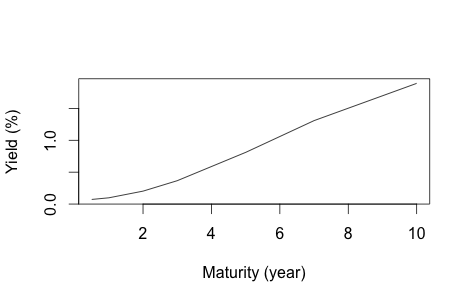
\includegraphics[width=0.75\textwidth]{fit.png}
    \end{center}
    \caption{Polynomial Regression of Yield Rates}
\label{fig:yield}
\end{figure}
\\Then we calculate the present value of the liability streams with the formula presented in the foregoing chapter.
 $$ pv=\sum_{i=1}^{2n} \frac{x_i}{(1+\frac{r_i}{2})^i} $$ 
The calculated present values of Poway school district's liability stream are listed in Table \ref{tab:pv}. Therefore, the total present value of the liability stream is 119.9 million dollars.
\begin{table}[htbp]
  \centering
  \caption{Present Value of Liability Stream}
    \begin{tabular}{|c|c|c|}
\hline
    Date  & Liability (M\$) & PV of liability from polynomial regression (M\$) \\\hline
    2012/7/15 & 6     & 6 \\
    2013/1/15 & 6     & 5.99 \\
    2013/7/15 & 9     & 8.98 \\
    2014/1/15 & 9     & 8.96 \\
    2014/7/15 & 10    & 9.93 \\
    2015/1/15 & 10    & 9.89 \\
    2015/7/15 & 10    & 9.84 \\
    2016/1/15 & 10    & 9.77 \\
    2016/7/15 & 8     & 7.76 \\
    2017/1/15 & 8     & 7.68 \\
    2017/7/15 & 8     & 7.6 \\
    2018/1/15 & 8     & 7.51 \\
    2018/7/15 & 6     & 5.56 \\
    2019/1/15 & 6     & 5.48 \\
    2019/7/15 & 5     & 4.5 \\
    2020/1/15 & 5     & 4.43 \\\hline
    Total   & 124   & 119.9 \\\hline
    \end{tabular}
  \label{tab:pv}
\end{table}
\newpage
\subsection{Asset Selection}
\vspace{8pt}
In our analysis procedure, a crucial part is selecting the appropriate assets. We will first choose around 30 assets to construct a portfolio to fulfill our future liability obligations. \\
\\
When making this final selection, we take three factors into consideration: credit risk, interest rate risk and payment matching.\\
\begin{itemize}
\item Credit Risk\\
\\
\noindent After reviewing different bonds types and their credit rating information, we decide to choose the bonds with minimum default risk for Poway Unified School District. Therefore, the assets we selected are all governmental bonds. Government bonds are usually referred to as risk-free bonds, because the government can raise taxes or create additional currency in order to redeem the bond at maturity. This ensures that all obligations will be fulfilled without default risks. Compared to other bonds issued by corporations or municipal governments, Treasury bonds can best fulfill this criterion.\\

\item Interest Rate Risk\\
\\
Another concern for choosing the assets is interest rate risk. Since we need to know portfolio future cash flow when we construct the portfolio, we need to choose bonds with fixed payments. In this way, we eliminate TIPS\footnote {TIPS is short for Treasury Inflation Protected Securities, and it is further explained in the appendix.}, which has adjustable principals. \\

\item Payment Matching\\
\\
The maturities for selected assets should match those of our liability. As presented, the payment is made semi-annually, so our assets should pay at around those dates. This is one reason we choose T-notes, which have regular semi-annual payments. To solve the problem that there is no matching bond on the exact days, we choose T-notes with maturity before the exact payment dates. Note that this is of great importance since if we choose ones after the dates, the notes will fail to meet the obligation.\\
\end{itemize}

\noindent Eventually, we find 32 assets satisfying the above criteria. The portfolio is made up of non-callable\footnote{Non-callable means the financial security cannot be redemmed early by the issuer, usually the non-callable securities tend to pay a lower interest rate than callable securities.} Treasury-notes and Treasury-bonds, mostly with coupons.\footnote{\noindent The data is gathered from Yahoo!~Finance.} The portfolio assets are shown in Table \ref{tab:tnote}, where the price, coupon rate and maturity date of each bond are given. \\
\\
\newpage
\begin{table}[h]
\centering
    \begin{tabular}{|c|c|c|c|}
 \hline
    \textbf{Issue} & \textbf{Price} & \textbf{Coupon(\%)} & \textbf{Maturity} \\\hline
    \textbf{T-NOTE 0.625} & 100   & 0.625 & 30-Jun-12 \\\hline
    \textbf{T-NOTE 1.500} & 102   & 1.5   & 15-Jul-12 \\\hline
    \textbf{T-NOTE 0.625} & 100   & 0.625 & 31-Dec-12 \\\hline
    \textbf{T-NOTE 1.375} & 101   & 1.375 & 15-Jan-13 \\\hline
    \textbf{T-NOTE 3.375} & 106   & 3.375 & 30-Jun-13 \\\hline
    \textbf{T-NOTE 1.000} & 101   & 1     & 15-Jul-13 \\\hline
    \textbf{T-NOTE 0.750} & 99.4  & 0.75  & 15-Dec-13 \\\hline
    \textbf{T-NOTE 1.500} & 101   & 1.5   & 31-Dec-13 \\\hline
    \textbf{T-NOTE 2.250} & 103   & 2.25  & 31-May-14 \\\hline
    \textbf{T-NOTE 2.625} & 104   & 2.625 & 30-Jun-14 \\\hline
    \textbf{T-NOTE 2.125} & 102   & 2.125 & 30-Nov-14 \\\hline
    \textbf{T-NOTE 2.625} & 104   & 2.625 & 31-Dec-14 \\\hline
    \textbf{T-NOTE 2.125} & 102   & 2.125 & 31-May-15 \\\hline
    \textbf{T-NOTE 1.875} & 101   & 1.875 & 30-Jun-15 \\\hline
    \textbf{T-NOTE 1.375} & 97.5  & 1.375 & 30-Nov-15 \\\hline
    \textbf{T-NOTE 2.125} & 101   & 2.125 & 31-Dec-15 \\\hline
    \textbf{T-NOTE 3.250} & 105   & 3.25  & 31-May-16 \\\hline
    \textbf{T-NOTE 3.250} & 105   & 3.25  & 30-Jun-16 \\\hline
    \textbf{T-NOTE 2.750} & 102   & 2.75  & 30-Nov-16 \\\hline
    \textbf{T-NOTE 3.250} & 105   & 3.25  & 31-Dec-16 \\\hline
    \textbf{T-NOTE 2.750} & 101   & 2.75  & 31-May-17 \\\hline
    \textbf{T-NOTE 2.500} & 99.8  & 2.5   & 30-Jun-17 \\\hline
    \textbf{T-NOTE 2.250} & 97.4  & 2.25  & 30-Nov-17 \\\hline
    \textbf{T-NOTE 2.750} & 100   & 2.75  & 31-Dec-17 \\\hline
    \textbf{T-BOND 9.125} & 142   & 9.125 & 15-May-18 \\\hline
    \textbf{T-NOTE 3.875} & 107   & 3.875 & 15-May-18 \\\hline
    \textbf{T-BOND 9.000} & 142   & 9     & 15-Nov-18 \\\hline
    \textbf{T-NOTE 3.750} & 106   & 3.75  & 15-Nov-18 \\\hline
    \textbf{US TREASURE} & 77.5  & 0     & 15-May-19 \\\hline
    \textbf{T-NOTE 3.125} & 101   & 3.125 & 15-May-19 \\\hline
    \textbf{US TREASURE} & 75.3  & 0     & 15-Nov-19 \\\hline
    \textbf{T-NOTE 3.375} & 102   & 3.375 & 15-Nov-19 \\\hline
    \end{tabular}
  \caption{Portfolio Assets}
  \label{tab:tnote}
\end{table}


\subsection{Cash Flow Matching}


In this section, we are going to conduct quantitative analysis about cash flow matching and immunization. Specifically we will construct a dedicated portfolio that can generate future cash flow to satisfy our future financial obligation.\\
\\
We plug data into the linear programming system:
\begin{eqnarray*}
\textrm{minimize}\quad    c^T x &   &    \\
\textrm{subject to}\quad  Ax    & \geq& b   \\
                  \mathbf{1}^T x & = & 1\\
                     x     & \geq &0
\end{eqnarray*} where each mathematical symbol has been explained in the Chapter of Technical Background 3.3.
Then the rest of work is to solve the linear programming. After optimization, our initial cost is 112.21 million dollars. Here we do not need further research into the asset allocation details because immunization will change the weights and provide a relatively riskless portfolio.

\subsection{Immunization}
\vspace{8pt}

Immunization locks in a fixed rate of return during the amount of time an investor plans to keep the bond without cashing it in.\\
\\
To immunize a bond portfolio, we need to know the duration of the bonds in the portfolio and adjust the portfolio so that the portfolio's duration equals the investment time horizon. For example, suppose we need to have \$50,000 in five years for your child's education. We might decide to invest in bonds. We can immunize our bond portfolio by selecting bonds that will equal exactly \$50,000 in five years regardless of interest rate changes. We can buy one zero-coupon bond that will mature in five years to equal \$50,000, or several coupon bonds each with a five year duration, or several bonds that ``average" a five-year duration.\\
\\
In our project, the linear program is set up to minimize total price of the bond portfolio by changing non-negative weight of each bond under the constraints that duration, present value of the bond portfolio are equal to those of the liability stream.\\
\\
The mathematical form of this linear program has been given in the Chapter of Technical Background 3.4.\\
\\
The features of targeted liability stream is listed in Table \ref{tab:bp}.\\
\begin{table}[h]
\centering  
\begin{tabular}{|c|c|}
\hline
Feature  &Amount\\ \hline  
Total Price  &113.2814 million dollars\\
Total Duration  &7.85432 years\\ 
Total Present Value  &119.8625 million dollars\\ 
\hline
\end{tabular}
\caption{Bond Portfolio}
\label{tab:bp}
\end{table}

\noindent By solving the linear program, we get the initial cost to be 113.28 million dollars. In summary, our optimized portfolio, priced at 113.28 million dollars in the same unit as the liability stream, is composed of 0.126 Treasury note expiring on June 30, 2012, with a coupon rate of 62.5 bps; 0.488 Treasury note expiring on November 30, 2015, with a coupon rate of 137.5 bps; and 0.386 Treasury bond expiring on November 15, 2018, with a coupon rate of 375 bps. \\

\chapter{Results}
After going through the procedures of our research, we get the following results.
\begin{itemize}
\item The total present value of Poway school district's liability stream is 119.9 million dollars, based on the predicted yield curve we've obtained from polynomial regression.
\item The qualitative process of asset selection presents the bond pool listed in Table \ref{tab:tnote}.
\item The process of cash flow matching generates a bond portfolio with initial value 112.21 million dollars.
\item The immunization model presents us a dedicated bond portfolio priced at 113.28 million dollars in the same unit as the liability stream. In detail, the portfolio is composed of 0.126 Treasury note expiring on June 30, 2012, with a coupon rate of 62.5 bps; 0.488 Treasury note expiring on November 30, 2015, with a coupon rate of 137.5 bps; and 0.386 Treasury bond expiring on November 15, 2018, with a coupon rate of 375 bps.
\end{itemize}


\chapter{Conclusions}\label{}
		        
Here, we will make conclusions with respect to our expected delieverables to our sponsor at the beginning of our project.
\begin{itemize}
\item The R package:\vspace{1mm}
\\
Our R package for calculating the present value proved to be sufficiently accurate in terms of either choosing the order of polynomial curve or the actual calculation.\\
\item The list of assets we choose for the portfolio:\vspace{1mm}
\\
The immunization model presents us a dedicated bond portfolio priced at 113.28 million dollars in the same unit as the liability stream. In detail, the portfolio is composed of 0.126 Treasury note expiring on June 30, 2012, with a coupon rate of 62.5 bps; 0.488 Treasury note expiring on November 30, 2015, with a coupon rate of 137.5 bps; and 0.386 Treasury bond expiring on November 15, 2018, with a coupon rate of 375 bps.\\
\\
The low risk of our assets, which are either treasury notes and treasuty bonds, provides the best steady cash inflow insurance with very small volatility. Actually we could simply consider our portfolio as riskless. Because we only have three nontrivial constraints and three instruments, whereas in cash flow matching we have an overloaded program requiring a dozen kinds of bonds for the solution.\\
\item The performance of the our portfolio:\vspace{1mm}
\\
Our immunization strategy is proved to be appropriate. Immunization, if possible and complete, can protect against term mismatch but not against other kinds of financial risk such as default by the borrower. By choosing duration as the major factors to consider when doing linear programming, we've generated an almost perfectly fit portfolio to cover the semiannual payments. One minor disadvantage associated with duration matching is that it assumes the durations of assets and liabilities remain unchanged, which is rarely the case.\\
    \item Constructive suggestions for improvement:\vspace{1mm}
\\
We have suggestions for Poway Unified School District Council. It is necessary to rebalance or reimmunize the portfolio from time to time since the duration depends on yield. The immunization method assumes that all yields are equal which is not quite realistic to have bonds with different maturities to have the same yield. Therefore, when the prevailing interest rate changes, it is unlikely that the yields on all bonds all change by the same amount. Only by rebalancing or reimmunizing can Poway Unified School District keep their liability stream well secured. \\
\end{itemize}
\noindent In summary, we are confident that given the current market information, our approach is sufficient to offer a reliable bond portfolio at a minimum cost but with maximum degree of matching with the bond stream obligation each period. If given more market information, we are confident to rule out more risk coming with this portfolio. Therefore, we successfully design the strategy for our sponsor, Stone \& Youngberg, to construct a dedicated portfolio that can generate future cash flow to satisfy Poway school district's future financial obligations. 



\appendix
\ifthenelse{\boolean{@twoside}}{\myclearpage}{}
\chapter{Programming Code}\label{Programming Code}
\section{Yield Curve Calculation}
\begin{itemize}
\item Yield curve predication:
\\

\begin{lstlisting}
yield=function(m=NULL,y=NULL)
{ 
  p = lm(y~poly(m,3))
  plot(m,predict(p,data.frame(m)),type=``l",xlab=``Maturity (year)",
  ylab``Yield (%)")  
#fitted value for different time in a year
  return(predict(p,data.frame(m)))
}
\end{lstlisting}
\vspace{8pt}
\item Calculation with real data:\\
We obtained daily treasury yield curve rates from the website of United States Department of Treasury. \footnote{Data Source: \\
http://www.treasury.gov/resource-center/data-chart-center/interest-rates/Pages/TextView.aspx?data=yield}\\
\\
The datasets obtained can be plugged into the R function of yield curve calculation listed as below. The R code below can directly generate a data file.\\

\begin{lstlisting}
maturity =c(0.5,1,2,3,5,7,10)
yi = c(0.06,0.10,0.24,0.34,0.80,1.32,1.89)
 #The bond yields obtained on 01/13/12 (percent), the resource is 
described as in the footnote.
predicted_yield=data.frame(Predicted_Yield=yield(maturity,yi))
save(file=`predicted_yield.RData',list=`predicted_yield')

\end{lstlisting}
\end{itemize}

\section{Linear Programming}
\begin{itemize}
\item R code for solving linear programs:\\
We build a ``lpsove" function in our R package to solve the two linear programs in our project. We construct the linear programs and plug in the bond prices, present values, durations, and match them with those of the liability stream. This function requires the R package named ``lpSolve".\\

\begin{lstlisting}
  
lpsolve=function(direction = "min", objective.in, const.mat, const.dir, const.rhs){
  require("lpSolve",character.only=TRUE)
  lpsolve=lp (direction, objective.in, const.mat, const.dir, const.rhs
            )
  return (lpsolve)}

\end{lstlisting}
\end{itemize}

\chapter{Glossary}\label{Glossary}

\vspace{12pt} 

\vspace{8pt}
\noindent {\bf Cash Flow Matching}. The strategy used to construct a portfolio that will fund a schedule of liabilities from a portfolio's cash flows, with the portfolio's value diminishing to zero after payment of the last liability. 

\vspace{8pt}
\noindent {\bf Immunization}. A hybrid strategy having elements of both active and passive strategies . It's used to minimize reinvestment risk over a specified investment horizon.\\
There are three necessary conditions to assure multiple liability immunization:
1) Present value of the assets must equal the present value of the liabilities
2) The composite portfolio duration must equal the composite liabilities duration
3) The distribution of durations of individual assets in the portfolio must have a wider range than the distribution of the liabilities


\vspace{8pt} \noindent {\bf Duration}. In finance, the duration of a financial asset that consists of fixed cash flows, for example a bond, is the weighted average of the times until those fixed cash flows are received. When an asset is considered as a function of yield, duration also measures the price sensitivity to yield, the rate of change of price with respect to yield or the percentage change in price for a parallel shift in yields.

\vspace{8pt} \noindent {\bf TIPS}. A treasury security that is indexed to inflation in order to protect investors from the negative effects of inflation. TIPS are considered an extremely low-risk investment since they are backed by the U.S. government and since their par value rises with inflation, as measured by the Consumer Price Index, while their interest rate remains fixed. Interest on TIPS is paid semiannually.

\ifthenelse{\boolean{@twoside}}{\myclearpage}{}

%\endinput

% Add your bibliography to Contents
\ifthenelse{\boolean{@twoside}}{\myclearpage}{\newpage}



\newpage
\begin{thebibliography}{4}  
\bibitem{} Menchero, Jose and Benjamin Davis, 2007, ``Risk Contribution is Exposure Times Volatility Times Correlation," \emph{The Journal of Portfolio Management, 37(1).} 
\bibitem{}  Winkelmann, Kurt, Scott McDermott, Alain Kerneis and Yevgenia Zemlyakova, 2007, ``Liability-Driven Investment Policy: Structuring the Hedging Portfolio," \emph{Goldman Sachs Asset Management Strategic Research.}
\bibitem{}  Ross, S., 1976, ``Options and Efficiency," \emph{Quarterly Journal of Economics, 90.}
\bibitem{}  Bates, D., 2001, ``The Market for Crash Risk," \emph{University of Iowa.}
\end{thebibliography}


\end{document}
